\chapter[Metodologia]{Metodologia}

Este capítulo apresenta os procedimentos metodológicos utilizados no desenvolvimento do trabalho. São descritas a classificação da pesquisa, as fontes e os recortes analíticos, a arquitetura do pipeline em Python, as regras de transformação por indicador, os mecanismos de rastreabilidade e validação, a modelagem dimensional da camada Gold e a disponibilização dos dados no Power BI.

\section{Classificação da pesquisa}

Este trabalho caracteriza-se como uma pesquisa aplicada, pois teve como finalidade desenvolver uma solução computacional baseada em Engenharia de Dados e Business Intelligence para organizar, integrar e analisar indicadores educacionais brasileiros \cite{prodanov2013}.

Quanto aos objetivos, a pesquisa classifica-se como descritiva, uma vez que buscou organizar, representar e analisar características relacionadas aos indicadores da Educação Básica brasileira, identificando comportamentos, padrões e variações presentes nos dados ao longo do tempo \cite{gil2002}.

Em relação à abordagem, a pesquisa caracteriza-se como quantitativa, pois utilizou bases de dados estruturadas e indicadores numéricos para realização das análises. As informações foram tratadas por meio de técnicas computacionais, permitindo a criação de métricas, comparações históricas, médias, proporções e representações gráficas \cite{prodanov2013}.

Quanto aos procedimentos técnicos, caracteriza-se como pesquisa documental, pois utiliza dados secundários disponibilizados por instituição oficial, sem intervenção direta sobre o ambiente analisado \cite{gil2002}. O desenvolvimento inclui ainda a construção de um artefato computacional, composto pelo pipeline de dados, modelo dimensional, medidas semânticas e dashboards.

\section{Fontes e coleta dos dados}

Foram utilizadas bases públicas disponibilizadas pelo Instituto Nacional de Estudos e Pesquisas Educacionais Anísio Teixeira (INEP): IDEB, SAEB, Taxas de Rendimento Escolar, Taxa de Distorção Idade-Série (TDI) e Prova Nacional Docente (PND) 2025.

A análise histórica compreende o período de 2007 a 2023 para IDEB, SAEB, Rendimento Escolar e TDI, com foco na rede pública e nos Anos Iniciais e Anos Finais do Ensino Fundamental. O Ensino Médio não integra o recorte final. A PND é tratada separadamente, apenas para 2025, e não compõe a série histórica principal.

Os links oficiais do INEP constituem a referência institucional e a fonte primária dos dados. Os arquivos armazenados localmente na camada Raw correspondem aos materiais obtidos dessas fontes e são identificados em manifesto por caminho local, finalidade e hash SHA-256. O inventário utilizado no projeto contém 54 arquivos e pode ser verificado pelo comando \texttt{python scripts/gerar\_manifesto\_raw.py --check}. A cópia organizada da Raw disponibilizada fora do repositório constitui apenas uma conveniência de reprodução e não substitui as fontes oficiais.

\section{Arquitetura e processo de extração}

A solução foi organizada em quatro camadas de dados, seguidas pela camada de consumo analítico:

\begin{center}
\texttt{RAW $\rightarrow$ BRONZE $\rightarrow$ SILVER $\rightarrow$ GOLD $\rightarrow$ POWER BI}
\end{center}

A Raw preserva os insumos oficiais organizados localmente. A Bronze realiza a ingestão com padronização técnica mínima e preservação de metadados. A Silver aplica o recorte analítico, harmonização de categorias, seleção das observações e validações de correspondência com a Bronze. A Gold materializa as tabelas fato e dimensão consumidas pelo Power BI.

Os arquivos de origem apresentam formatos heterogêneos, incluindo \texttt{.xls}, \texttt{.xlsx}, \texttt{.xlsb}, \texttt{.csv} e \texttt{.txt}. A leitura e o processamento são executados por scripts Python. O orquestrador \texttt{src/pipeline.py} organiza as etapas de Bronze, Silver, Gold e validação global e disponibiliza, entre outros, os comandos \texttt{bronze}, \texttt{silver}, \texttt{gold}, \texttt{validate-gold} e \texttt{full}, além do modo \texttt{--dry-run} para inspeção da sequência sem execução analítica.

A nomenclatura local da Raw segue uma regra condicional. Quando o nome original do arquivo já apresenta explicitamente o ano de referência, ele é preservado. Quando o ano não está explícito, ele pode ser acrescentado localmente para facilitar a organização temporal, sem alterar conteúdo, estrutura ou valores. O IDEB constitui uma exceção intencional: o projeto utiliza um único arquivo local canônico na pasta \texttt{data/raw/ideb}, denominado \texttt{divulgacao\_regioes\_ufs\_ideb.xlsx}, independentemente do ano presente no nome da edição oficial baixada.

\section{Transformação, linhagem e validação}

As transformações foram implementadas em Python de acordo com as particularidades de cada fonte. Entre os procedimentos aplicados estão identificação de cabeçalhos técnicos, padronização de tipos, normalização de Unidades Federativas, tratamento de valores ausentes, harmonização de categorias, seleção de rede e etapa, transformação entre formatos amplo e longo quando necessária e validação do grão analítico.

A rastreabilidade é preservada ao longo do pipeline. Na Bronze são mantidos metadados técnicos associados à fonte, ao hash, ao nome do arquivo e à aba de origem, ao ano de referência, à posição das linhas e à granularidade preservada, conforme aplicável. Na Silver, os registros analíticos são validados diretamente contra suas células de origem por arquivo, linha e coluna; no IDEB e no SAEB, também são consideradas aba e granularidade quando pertinentes. Essa estratégia permite relacionar um valor analítico à observação de origem utilizada em sua construção.

As informações de rede são selecionadas segundo a semântica de cada fonte, sem calcular indiscriminadamente média entre redes federal, estadual e municipal. Rendimento e TDI utilizam o agregado público oficial; o IDEB seleciona a categoria pública disponibilizada no arquivo; e o SAEB aplica regras específicas por edição. A rede privada é excluída. No SAEB de 2007 e 2009, a categoria histórica disponível corresponde a \texttt{Total - Estadual e Municipal}, particularidade considerada como limitação de comparabilidade da série.

As validações abrangem esquema, domínios, quantidade de registros, unicidade no grão, cobertura temporal e territorial, correspondência entre camadas, chaves órfãs e consistência dos relacionamentos. Na Gold, o validador global verifica também a integridade referencial e a coerência entre município e UF na PND.

\subsection{Tratamento da base IDEB}

O IDEB utiliza um único arquivo Raw canônico de divulgação por Regiões e Unidades da Federação. A versão física corrente do arquivo pode conter colunas de edições posteriores, inclusive 2025, mas a Silver e a Gold desta versão selecionam deliberadamente as nove edições de 2007 a 2023: 2007, 2009, 2011, 2013, 2015, 2017, 2019, 2021 e 2023. Assim, a atualização física da fonte não amplia automaticamente o escopo analítico.

A tabela final \texttt{FATO\_IDEB} contém \texttt{ANO}, \texttt{UF}, \texttt{ETAPA}, \texttt{REDE} e \texttt{IDEB}. O Ensino Médio é excluído, mantendo apenas Anos Iniciais e Anos Finais da rede pública.

\subsection{Tratamento da base SAEB}

A série final do SAEB utiliza resultados oficiais agregados por Unidade Federativa para as nove edições entre 2007 e 2023. As disciplinas são harmonizadas em Língua Portuguesa e Matemática. Arquivos escolares e microdados permanecem no projeto para auditoria e rastreabilidade, mas não constituem a regra geral de cálculo da fato final.

Uma auditoria específica de 2023 comparou o agregado oficial com reconstruções baseadas em escolas. Como nem a média simples nem a média ponderada por participantes reproduziram os valores oficiais de UF, o projeto preservou o resultado agregado publicado pelo INEP. A \texttt{FATO\_SAEB} final contém \texttt{ANO}, \texttt{UF}, \texttt{ETAPA}, \texttt{REDE}, \texttt{DISCIPLINA} e \texttt{PROFICIENCIA}.

\subsection{Tratamento da base de Rendimento Escolar}

O Rendimento Escolar utiliza 17 arquivos anuais, de 2007 a 2023, obtidos no item oficial referente a Brasil, regiões e UFs. Os layouts variam entre períodos e são tratados por configurações específicas em Python. A seleção analítica utiliza o agregado público oficial e as etapas Anos Iniciais e Anos Finais.

A tabela \texttt{FATO\_RENDIMENTO} contém \texttt{ANO}, \texttt{UF}, \texttt{ETAPA}, \texttt{REDE}, \texttt{INDICADOR} e \texttt{VALOR}. Os indicadores \texttt{APROVACAO}, \texttt{REPROVACAO} e \texttt{ABANDONO} compartilham a mesma estrutura factual.

\subsection{Tratamento da base de Distorção Idade-Série}

A TDI também utiliza 17 arquivos anuais, de 2007 a 2023, referentes a Brasil, regiões e UFs. Após a harmonização dos diferentes layouts, a saída analítica é consolidada na \texttt{FATO\_TDI}, com as colunas \texttt{ANO}, \texttt{UF}, \texttt{ETAPA}, \texttt{REDE} e \texttt{TDI}.

A TDI permanece na escala de 0 a 100. As medidas temporais calculadas no Power BI não pressupõem que todas as fontes tenham observação em todos os anos; para cada indicador, a variação utiliza o primeiro e o último ano com dado dentro do intervalo selecionado.

\subsection{Tratamento da base PND 2025}

A PND 2025 foi incorporada como análise complementar. O arquivo de microdados possui 1.087.359 registros. A auditoria identificou 759.152 registros com os cinco resultados analíticos completos; 759.140 desses registros também atendem ao critério \texttt{TP\_PRES = 555} e constituem a população analítica. Permanecem fora 966 registros presentes sem o conjunto completo de resultados e 12 registros com \texttt{TP\_PRES = 888} apesar de apresentarem resultados completos.

A Gold preserva \texttt{UF\_PROVA} e \texttt{CO\_MUNICIPIO\_PROVA}, que representam o local de aplicação da prova e não a residência do participante. Também preserva o código de área \texttt{CO\_GRUPO}, as notas e resultados analíticos e o campo \texttt{PADRAO\_DESEMPENHO}. O código municipal é relacionado à \texttt{DIM\_MUNICIPIO}; a Gold não incorpora nome de município na fato.

A classificação de desempenho é baseada exclusivamente na nota objetiva. A Nota Técnica nº 44/2025/CEI/CGGI/DAES-INEP documenta a transformação da proficiência objetiva para a escala de divulgação de \texttt{NT\_OBJ}, e a Nota Técnica nº 1/2026/GPP/GAB-INEP estabelece os pontos de corte utilizados na PND por meio do método de Angoff Modificado \cite{inep2025notatecnica44,inep2026notatecnica1}. O projeto aplica:

\begin{center}
\texttt{NT\_OBJ < 50 $\rightarrow$ NAO\_PROFICIENTE}\\
\texttt{50 $\leq$ NT\_OBJ < 70 $\rightarrow$ PADRAO\_1}\\
\texttt{NT\_OBJ $\geq$ 70 $\rightarrow$ PADRAO\_2}
\end{center}

Os grupos \texttt{PADRAO\_1} e \texttt{PADRAO\_2} compõem a medida de proficientes. Essa classificação não representa aprovação ou reprovação e o corte de 50 pontos não deve ser interpretado como 50\% de acertos.

\section{Modelagem dos dados}

Após as transformações, a camada Gold materializa cinco tabelas fato e cinco dimensões para consumo analítico. As fatos são \texttt{FATO\_RENDIMENTO}, \texttt{FATO\_TDI}, \texttt{FATO\_IDEB}, \texttt{FATO\_SAEB} e \texttt{FATO\_PND}. As dimensões são \texttt{DIM\_UF}, \texttt{DIM\_TEMPO}, \texttt{DIM\_ETAPA}, \texttt{DIM\_AREA\_PND} e \texttt{DIM\_MUNICIPIO}.

Os relacionamentos seguem cardinalidade 1:* e filtro unidirecional da dimensão para a fato. \texttt{DIM\_UF} relaciona-se com as cinco fatos; \texttt{DIM\_TEMPO}, também. \texttt{DIM\_ETAPA} relaciona-se apenas com as quatro fatos históricas. Para a PND, os relacionamentos adicionais utilizam \texttt{DIM\_AREA\_PND} e \texttt{DIM\_MUNICIPIO}. Não existe relação física direta entre \texttt{DIM\_UF} e \texttt{DIM\_MUNICIPIO}, evitando um segundo caminho geográfico até a \texttt{FATO\_PND}.

\begin{landscape}
\begin{figure}[H]
   \centering
   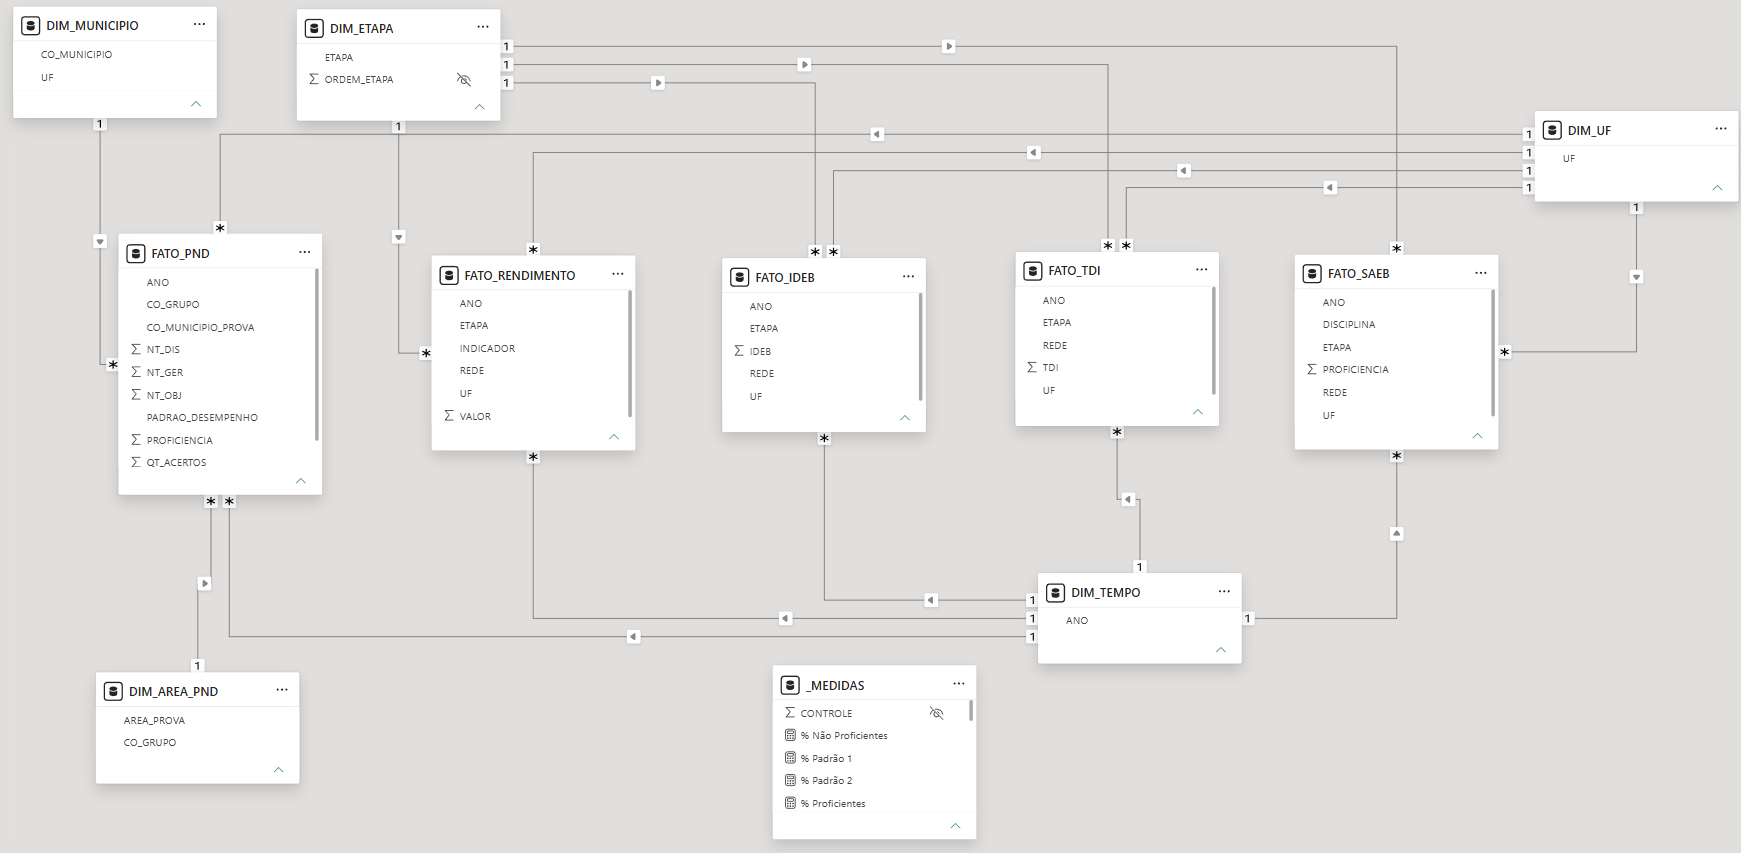
\includegraphics[width=0.95\linewidth]{figs/modelo-dimensional.png}
   \caption{Modelo dimensional atual consumido pelo Power BI.}
   \label{fig:modelo-dimensional}
\end{figure}
\end{landscape}

Na Figura~\ref{fig:modelo-dimensional}, a tabela \texttt{\_MEDIDAS} funciona apenas como contêiner técnico para organizar as medidas DAX no modelo semântico. Ela não constitui uma sexta dimensão nem uma tabela fato analítica.

\section{Desenvolvimento das métricas analíticas}

O modelo semântico possui 27 medidas DAX. As medidas calculam médias, taxas, contagens, proporções, apoio à seleção de anos comparáveis e variações temporais. A Tabela~\ref{tab:medidas-dax} resume os nomes implementados no arquivo \texttt{powerbi/medidas\_power\_bi.dax}.

\begin{table}[H]
\centering
\scriptsize
\caption{Medidas DAX implementadas no modelo semântico.}
\label{tab:medidas-dax}
\renewcommand{\arraystretch}{1.2}
\begin{tabular}{|p{3.0cm}|p{10.0cm}|}
\hline
\textbf{Grupo} & \textbf{Medidas} \\ \hline
Rendimento & \texttt{Taxa de Aprovação}; \texttt{Taxa de Reprovação}; \texttt{Taxa de Abandono} \\ \hline
TDI e IDEB & \texttt{TDI Média}; \texttt{IDEB Médio} \\ \hline
SAEB & \texttt{Proficiência Média SAEB}; \texttt{Proficiência Média LP}; \texttt{Proficiência Média MT} \\ \hline
PND -- médias e contagens & \texttt{Participantes PND}; \texttt{Nota Objetiva Média}; \texttt{Nota Discursiva Média}; \texttt{Nota Geral Média}; \texttt{Média de Acertos}; \texttt{Não Proficientes}; \texttt{Padrão 1}; \texttt{Padrão 2}; \texttt{Proficientes} \\ \hline
PND -- percentuais & \texttt{\% Proficientes}; \texttt{\% Não Proficientes}; \texttt{\% Padrão 1}; \texttt{\% Padrão 2} \\ \hline
Apoio & \texttt{Ano de Avaliação Disponível} \\ \hline
Variações & \texttt{Variação Aprovação}; \texttt{Variação IDEB}; \texttt{Variação SAEB Matemática}; \texttt{Variação SAEB Português}; \texttt{Variação TDI} \\ \hline
\end{tabular}
\legend{Fonte: Elaborado pelo autor a partir do modelo Power BI do projeto (2026).}
\end{table}

As taxas de Rendimento e a TDI já são armazenadas na escala de 0 a 100. Os percentuais da PND são razões calculadas dinamicamente e formatadas como percentuais. As medidas de variação representam diferença absoluta entre o último e o primeiro ano com dado no intervalo selecionado. Suas unidades dependem do indicador: pontos de IDEB, pontos percentuais para Aprovação e TDI e pontos de proficiência para SAEB.

\section{Desenvolvimento dos dashboards}

O Power BI consome exclusivamente os arquivos Parquet da Gold. O Power Query é utilizado como camada de conexão com esses arquivos; relacionamentos, medidas DAX e visualizações compõem o modelo semântico e a apresentação analítica.

A primeira página, \textit{Panorama dos Indicadores da Educação Básica}, reúne cartões de IDEB, proficiência média do SAEB em Matemática e Língua Portuguesa, Aprovação, Reprovação, Abandono e TDI, além das respectivas evoluções históricas.

A segunda página, \textit{Desempenho educacional por Unidade Federativa}, compara as UFs em quatro rankings: IDEB, SAEB Matemática, TDI e SAEB Língua Portuguesa. O ano é selecionado entre avaliações disponíveis para IDEB e SAEB, permitindo comparação territorial dentro de um mesmo recorte temporal.

A terceira página, \textit{Aprendizagem e fluxo escolar por Unidade Federativa}, combina a evolução histórica de Aprovação, Reprovação, Abandono e TDI com dois gráficos de dispersão: Aprovação versus IDEB e Aprovação versus proficiência média do SAEB.

A quarta página, \textit{Variação dos indicadores por Unidade Federativa}, utiliza um intervalo de anos e apresenta as diferenças entre o primeiro e o último ano com dado para IDEB, Aprovação, SAEB Língua Portuguesa e SAEB Matemática, respeitando as unidades próprias de cada indicador.

A quinta página, \textit{Distorção idade-série por Unidade Federativa}, apresenta TDI média e Variação TDI, evolução temporal, comparação por UF, comparação entre Anos Iniciais e Anos Finais e variação territorial.

A sexta página, \textit{Resultados da PND 2025}, apresenta os cartões \texttt{Participantes PND}, \texttt{\% Proficientes}, \texttt{Nota Objetiva Média} e \texttt{Nota Geral Média}. Os gráficos mostram percentual de proficientes por área, percentual de proficientes por UF, nota objetiva média por área e distribuição dos padrões de desempenho por UF. Os filtros visíveis dessa página são UF e área.

A sétima página, \textit{Metodologia e Arquitetura do Projeto}, sintetiza escopo, fontes, arquitetura Raw--Bronze--Silver--Gold--Power BI, modelo dimensional, decisões metodológicas e controles de qualidade. Ela funciona como documentação interna do próprio dashboard.

\begin{landscape}
\begin{figure}[H]
  \centering
  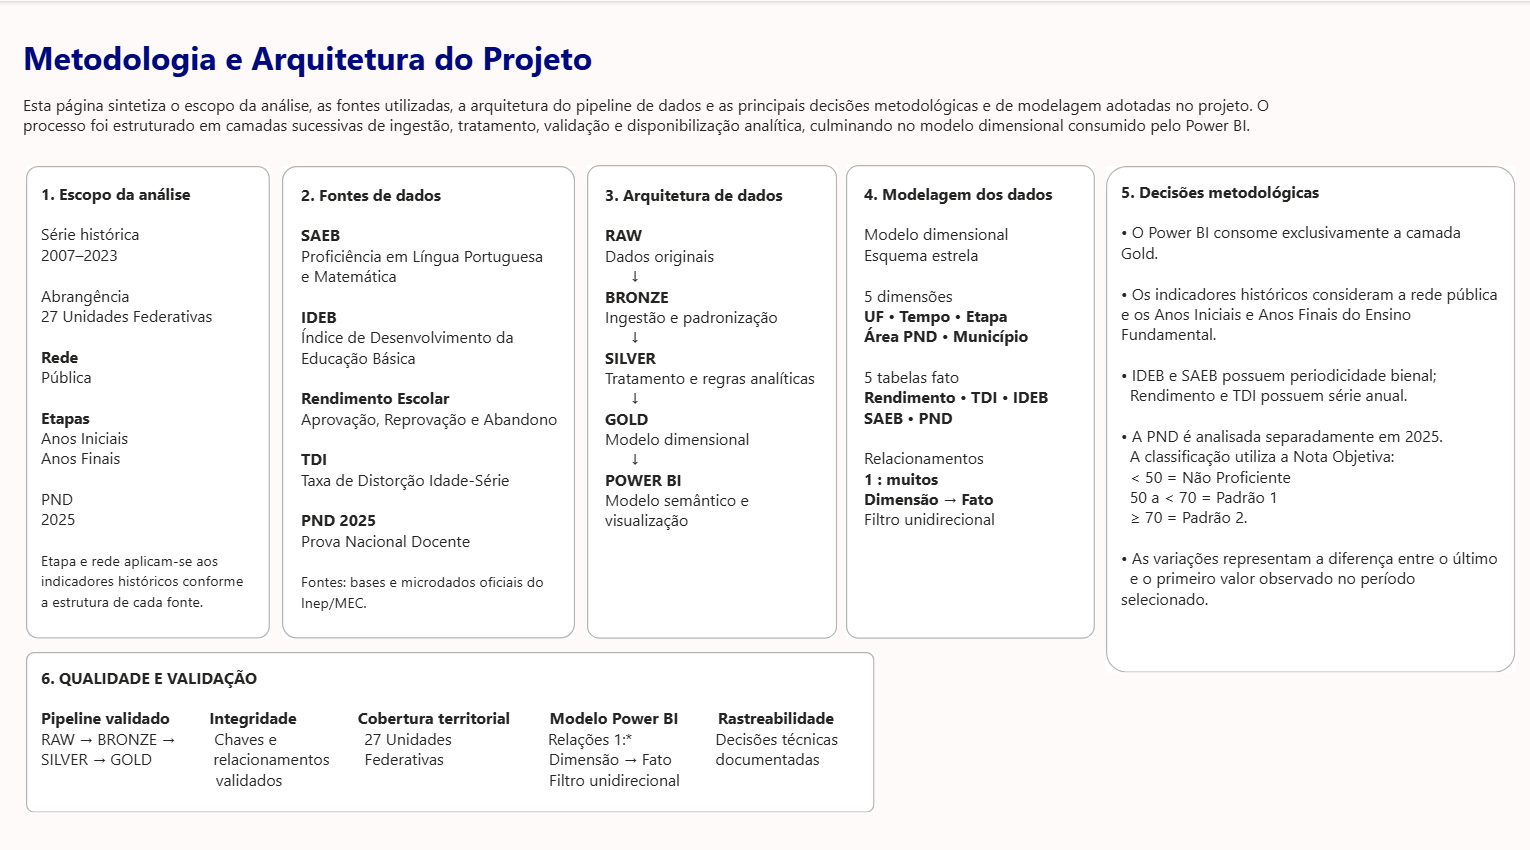
\includegraphics[width=0.95\linewidth]{figs/dashboard-metodologia.png}
  \caption{Página de metodologia e arquitetura do projeto no Power BI.}
  \label{fig:dashboard-metodologia}
\end{figure}
\end{landscape}

\section{Notebooks, testes e automação}

O repositório possui cinco notebooks demonstrativos, um para cada indicador: Rendimento Escolar, TDI, IDEB, SAEB e PND. Eles apresentam o percurso entre a fonte Raw e a tabela fato Gold correspondente e chamam os scripts oficiais do repositório, sem reimplementar as regras de transformação. Assim, os notebooks funcionam como material demonstrativo e executável da metodologia, enquanto a implementação oficial permanece em \texttt{src/}.

Além das validações analíticas, o projeto possui testes automatizados do contrato do repositório e um fluxo de integração contínua para verificações estruturais que não dependem da disponibilidade da Raw. O comando \texttt{python src/pipeline.py full --dry-run} valida a sequência de scripts sem executar as transformações, enquanto o manifesto pode ser verificado independentemente por \texttt{python scripts/gerar\_manifesto\_raw.py --check}.

\section{Ferramentas utilizadas}

Foram utilizadas Python e as bibliotecas registradas no arquivo \texttt{requirements.txt}, incluindo Pandas, NumPy, PyArrow e mecanismos de leitura de planilhas em diferentes formatos. Parquet foi adotado nas camadas derivadas para armazenamento tabular. Também foram utilizados Git para versionamento, notebooks Jupyter como material demonstrativo, Power BI Desktop para o modelo semântico e os dashboards, Power Query para conexão à Gold e DAX para as medidas analíticas.

Essa separação de responsabilidades mantém o processamento reprodutível fora da ferramenta de visualização: Python executa e valida o pipeline; os Parquets constituem a interface analítica; e o Power BI concentra relacionamentos, medidas dependentes do contexto de filtro e visualizações.

\section{Limitações metodológicas}
\label{sec:limitacoes-metodologicas}

As fontes apresentam diferenças históricas de formato, layout, nomenclatura, nível de agregação e semântica das categorias. Essas diferenças exigem regras específicas por indicador e por edição e limitam a interpretação de uma série como se todos os anos fossem metodologicamente idênticos.

A análise histórica é harmonizada principalmente no nível de Unidade Federativa, rede pública e Anos Iniciais/Anos Finais. Portanto, os resultados não devem ser generalizados para escolas ou municípios. No SAEB, as categorias de rede de 2007 e 2009 diferem das edições posteriores. IDEB e SAEB possuem periodicidade bienal, enquanto Rendimento e TDI são anuais.

As médias exibidas no Power BI são médias das linhas existentes no contexto de filtro. Quando diversas UFs são agregadas, esses valores não equivalem automaticamente a uma média nacional ponderada por matrículas ou participantes. Essa distinção é especialmente importante ao interpretar os cartões gerais.

A PND corresponde apenas a 2025 e não constitui série temporal. As variáveis territoriais representam o local de aplicação da prova, não residência. A classificação por padrões utiliza \texttt{NT\_OBJ} e descreve proficiência segundo os pontos de corte adotados; ela não equivale a aprovação ou reprovação.

A reprodução exata depende dos arquivos identificados no manifesto e pelos hashes SHA-256. Novas edições oficiais podem alterar nomes, layouts ou endereços de download, motivo pelo qual a documentação das fontes deve ser considerada em conjunto com o inventário versionado.

Por fim, os dashboards têm finalidade descritiva e exploratória. Associações visuais entre indicadores não permitem estabelecer relações causais nem atribuir mudanças observadas a políticas, condições socioeconômicas ou outros fatores sem desenho de pesquisa específico para inferência causal.
